% Faber2026 — CHIME/FRB–DSA-110 co-detected FRBs: dispersion & scattering budget
%
% Manuscript repo (Overleaf-synced). The analysis pipeline that produces the
% numbers and figures here is dsa110-FLITS, pinned as a git submodule under
% pipeline/ (see PIPELINE.md). Overleaf ignores the submodule and compiles
% the .tex / figures at the repo root.
\documentclass[twocolumn]{aastex631}

\usepackage{amsmath,amssymb}
\usepackage{graphicx}
\usepackage{placeins}
\graphicspath{{figures/}}

% Relax float placement for the figure-heavy co-detection sections.
\setcounter{topnumber}{5}
\setcounter{bottomnumber}{5}
\setcounter{totalnumber}{12}
\renewcommand{\topfraction}{0.95}
\renewcommand{\bottomfraction}{0.95}
\renewcommand{\textfraction}{0.05}
\renewcommand{\floatpagefraction}{0.85}
\extrafloats{24}

\begin{document}

\title{Scattering, Scintillation, and Energetics of Fast Radio Bursts
Codetected by CHIME/FRB and DSA-110}

% Author / affiliation block lives in auth.tex for reuse and clean diffs.
% Author block. Edit here; main.tex \input's this.
% No ORCID, affiliation, contact, or collaboration-approval claim is asserted.
\author{Jakob T. Faber}
\collaboration{1}{The CHIME/FRB Collaboration}
\collaboration{0}{The DSA-110 Collaboration}


\begin{abstract}
This circulation draft describes the planned joint dispersion- and
scattering-budget analysis of the CHIME/FRB--DSA-110 co-detection sample. The
central opportunity is the wide frequency baseline between CHIME/FRB
($0.4$--$0.8$\,GHz) and DSA-110 ($\sim$1.4\,GHz), which lets the analysis test
whether a single-band scattering interpretation survives when the pulse
broadening, frequency scaling, dispersion measure, and foreground environment
are constrained together. The draft lays out the association checks, dispersion
budget, foreground-census layer, two-band scattering model, scintillation
connection, and band-restricted energy calculation that will be used in the
final manuscript. It is intentionally conservative: previously generated fit,
foreground-census, dispersion-budget, association, DM-observation, scintillation,
and energy products are withheld until they pass the re-validation gates
described in the project context and circulation-readiness plan. As a result,
this version should be read as a collaborator-review draft of the argument,
scope, and analysis contract, not as a final presentation of citable numerical
results.
\end{abstract}

\keywords{Radio transient sources (2008) --- Interstellar scattering (854)
--- Intergalactic medium (813) --- Circumgalactic medium (1879)}

% \section*{Circulation-status note}
% 
% This draft is being circulated to check the manuscript structure, analysis
% contract, terminology, and missing collaborator inputs before the numerical
% results are restored. The current Results, Discussion, and Conclusions sections
% therefore mark which products are withheld rather than quoting values from the
% retired analysis campaign. Comments are most useful if they flag missing
% physical assumptions, unclear validation requirements, author-list corrections,
% or places where the eventual re-validated results need a different narrative
% slot.

\section{Introduction}
\label{sec:intro}

% TODO: FRB DM as a sum of Galactic, host, and cosmic contributions; scattering
% as a probe of turbulent ionized gas along the line of sight; the leverage of
% wide-baseline co-detection (CHIME/FRB at 400–800 MHz, DSA-110 at 1.4 GHz) for
% breaking the DM/scattering degeneracy; the question this paper answers — which
% medium contributes which observed feature, per sightline.

\section{Observations and Sample}
\label{sec:obs}

Our sample is the twelve fast radio bursts detected simultaneously by CHIME/FRB
\citep{CHIMEFRB2018} at $0.4$--$0.8$\,GHz and by DSA-110 \citep{Law2024} at
$\sim$1.4\,GHz between 2022 February and 2024 February (MJD $59617$--$60369$).
The defining asset of the sample is that each burst is seen twice across a
$\sim$1\,GHz frequency baseline, which---as developed in
Section~\ref{sec:jointfit}---breaks the degeneracy between the scattering time
and its spectral index that defeats any single-band fit. The bursts span a
dispersion measure range of $262$--$960$\,pc\,cm$^{-3}$; their nicknames, TNS
designations, epochs, widths, and time-of-arrival residuals are listed in
Table~\ref{tab:toa}. We report all twelve, noting per sightline the level at
which each quantity is constrained rather than imposing a single detection
threshold.

\subsection{Dynamic spectra and reduction}
\label{sec:data}

For each co-detection we analyze a pair of total-intensity dynamic spectra---one
per facility---derived from the CHIME/FRB and DSA-110 baseband recordings
(24 spectra in total; provenance and array geometry in
\texttt{DATA\_SOURCES.md} of the companion \texttt{dsa110-FLITS} archive). Each
spectrum is loaded with its frequency axis standardized to ascending order and
its per-channel bandpass normalized, so the fitted amplitudes are free of the
band-edge rolloff. All fits, quality gates, and figures in this paper are
produced by the open \texttt{dsa110-FLITS} pipeline (\texttt{pipeline/}), which
we reference throughout for reproducibility. We do not catalog the fine
baseband morphology of each burst here; the only morphological distinction the
analysis depends on---whether a burst resolves into more than one temporal
component---is treated where it matters, in the multi-component fit of
Section~\ref{sec:multicomp}.

\subsection{Scattering fits}
\label{sec:obs-scatt}

The joint CHIME--DSA fit yields a $1.4$\,GHz pulse-broadening time
$\tau_{1\,\mathrm{GHz}}$ wherever a scattering tail is resolved, measured against
the NE2001 Galactic prediction along the sightline. We fit the joint two-band
model across the co-detected sample with the turbulence spectral index $\beta$ as
the fundamental parameter, from which both the PBF shape and the frequency-scaling
index $\alpha=2\beta/(\beta-2)$ follow (Section~\ref{sec:jointfit}), modeling
temporal multiplicity per band (Sections~\ref{sec:results-alpha},
\ref{sec:disc-alpha}). Sightlines with interior posteriors return a measured
$(\tau_{1\,\mathrm{GHz}},\beta)$ pair; sightlines whose posterior rails at the
$\beta=4$ bound are consistent with the square-law (exponential-PBF) limit and
are quoted only as geometry-conditioned $\alpha=4$ limits, never as
measurements, while a posterior railing at the steep bound or failing the
quality gate is withheld entirely. The final per-sightline result of this
uniform re-fit is reported in Table~\ref{tab:beta} (eleven of twelve
sightlines; one gate failure), and Figure~\ref{fig:budget} overlays every
measured $\tau_{1\,\mathrm{GHz}}$ on the predicted intervening contribution
along its sightline (Section~\ref{sec:budget}).
Figure~\ref{fig:jointmodel_montage} shows the recovered joint model against the
DSA dynamic spectrum for every co-detection. Panels are ordered by burst
nickname; each pair is [data~|~model] on a common color scale, with the fitted
$\beta$ and DSA $\chi^2_\nu$ annotated. FRB~20220310F retains the dedicated
multiplicity demonstration of Figure~\ref{fig:whitney_mult}.

\begin{figure*}[!t]
  \centering
  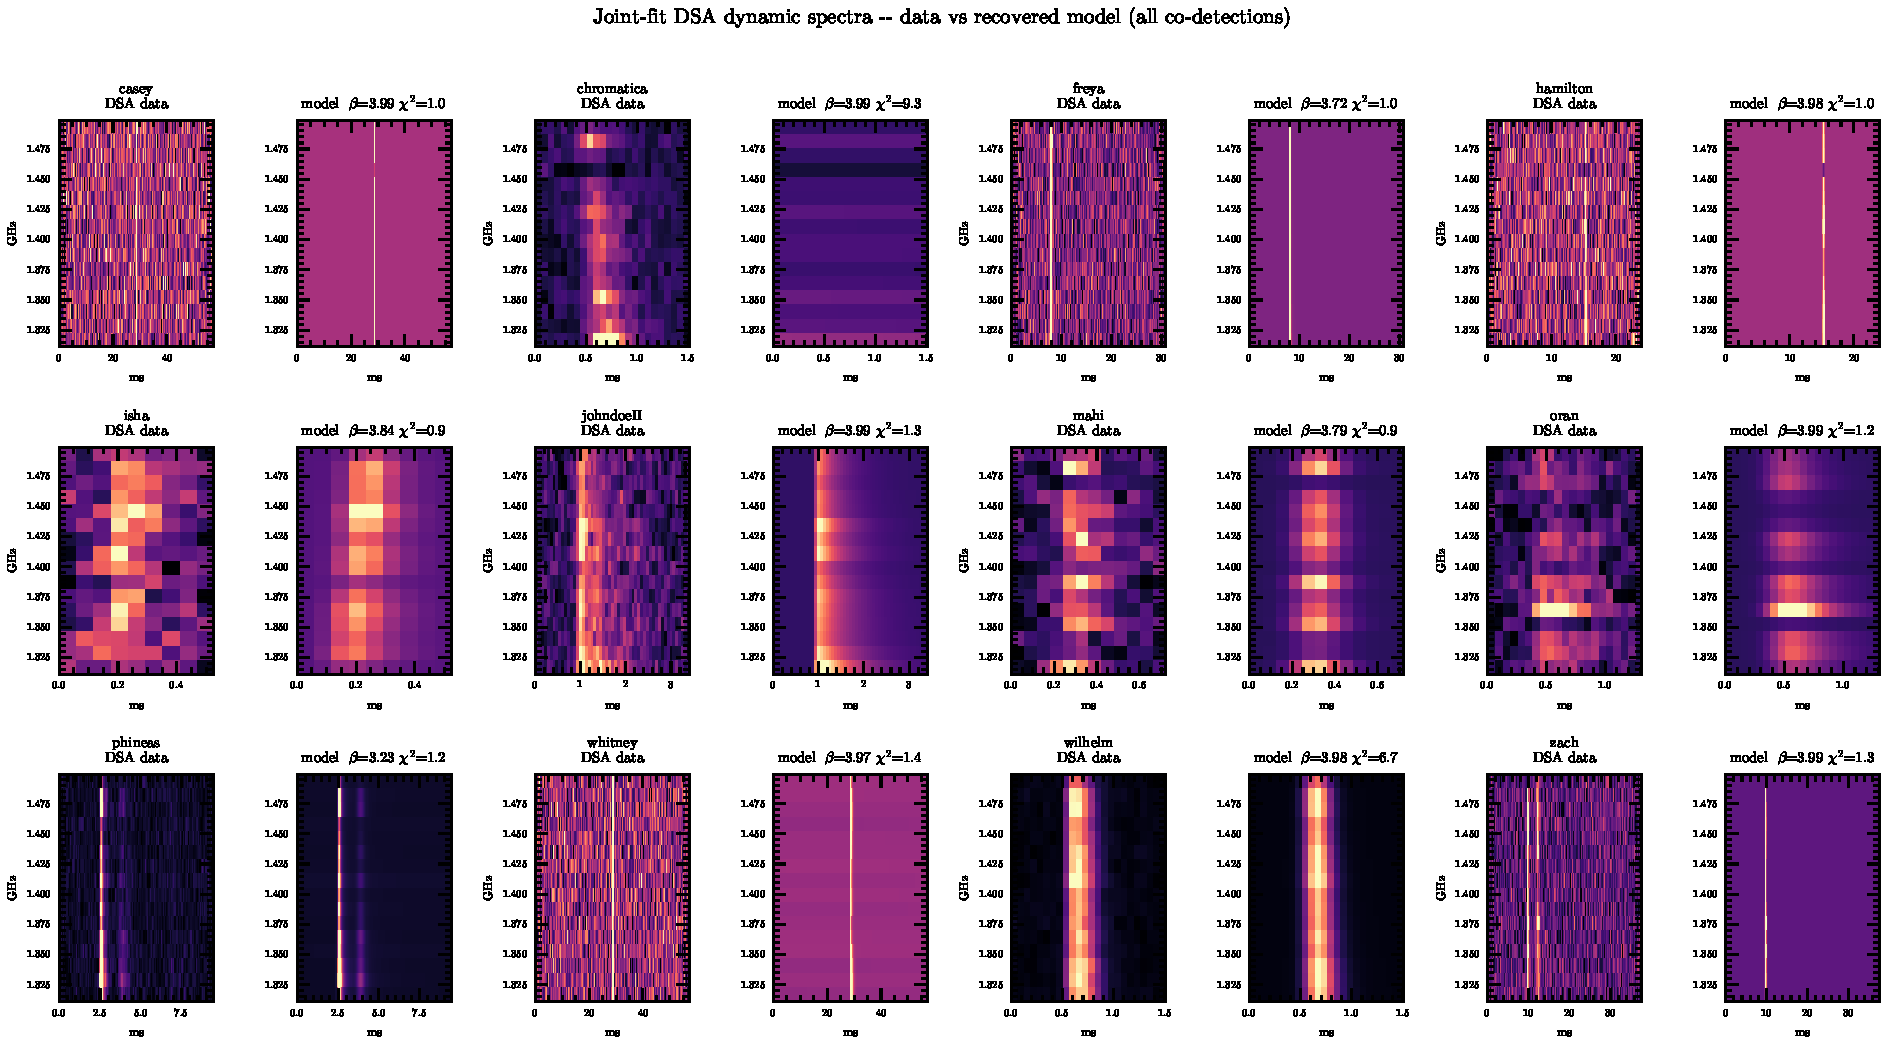
\includegraphics[width=\textwidth]{jointmodel_montage}
  \caption{Joint-fit model vs.\ data on the DSA-110 band for all twelve
  co-detections. Each row pair shows the on-pulse dynamic spectrum (left) and the
  gain-marginal model reconstruction (right) from the uniform $\beta$-based
  two-band fit (PBF shape and frequency scaling both derived from the fitted
  turbulence index $\beta$; Section~\ref{sec:jointfit}), at the per-burst
  component multiplicities of Table~\ref{tab:beta}. The fitted $\beta$ and
  DSA reduced $\chi^2$ are listed per panel; FRB~20220310F is shown with its
  committed two-component (C2D2) fit, whose multiplicity dependence is
  demonstrated in Figure~\ref{fig:whitney_mult}, and FRB~20240203A's flat
  model panel against strongly structured data visualizes its quality-gate
  failure (Table~\ref{tab:beta}). Rendered from the campaign joint fits by
  \texttt{dsa110-FLITS}
  (\texttt{analysis/scattering-refit-2026-06/plot\_jointmodel\_montage.py}).}
  \label{fig:jointmodel_montage}
\end{figure*}

\subsection{Foreground-galaxy search}
\label{sec:obs-fg}

To establish which sightlines could carry an intervening dispersion or
scattering contribution, we searched each of the twelve fields for foreground
galaxies and clusters, cross-matching candidates against the DESI Legacy Imaging
Survey DR9 with \citet{Zhou2021} photometric redshifts, DESI DR1 spectroscopic
redshifts, the NASA/IPAC Extragalactic Database, and PS1-STRM \citep{Beck2021}.
The search returns 49 candidate systems---34 galaxy halos and 15 clusters---along
nine of the twelve sightlines (three fields yield no candidate). For each
candidate we record the proper impact parameter (12--280\,kpc for the halos;
clusters by $b/R_{500}$) and the best available redshift and its provenance
(spectroscopic or photometric); the full catalog is Table~\ref{tab:foreground}.
Spectroscopic host redshifts are available for nine of the twelve bursts
($z=0.043$--$0.51$), while three (FRB 20230325A, FRB 20240122A, FRB 20230814B) carry only a
placeholder redshift and are excluded from any distance-dependent quantity. We measure no host stellar masses; the only masses entering the
analysis are the halo-mass proxies of the intervening systems used by the
circumgalactic dispersion model (Section~\ref{sec:dm}), whose confidence we flag
per system. The verdict logic that classifies each candidate as foreground,
background, or inconclusive, and the resulting dispersion budget, follow in
Section~\ref{sec:budget}.

\section{Methods}
\label{sec:methods}

This section defines how the co-detections are associated, how the
dispersion-measure and scattering budgets are modeled, and how the fitted
quantities used in Section~\ref{sec:results} are validated.

\subsection{Time-of-Arrival Crossmatching}
\label{sec:toa}

Before attributing the dispersion and scattering budgets we verify that the
twelve events are genuine co-detections---the same burst seen by both
facilities, with arrival times consistent under the cold-plasma dispersion law
and the geometric light-travel delay between the sites. The wide baseline
between CHIME/FRB (400--800\,MHz) and DSA-110 ($\sim$1.4\,GHz) makes the
co-detections a test of the $1/\nu^2$ dispersion scaling and of the relative
timing alignment of the two facilities \citep{Lorimer2007, Thornton2013}.

\subsubsection{Delay model}

We translate the arrival times at the two central frequencies to a common
reference frequency $\nu_{\mathrm{ref}}=400$\,MHz. The cold-plasma dispersion
delay is
\begin{equation}
\Delta t_p = K_{\mathrm{DM}}\,\mathrm{DM}
\left(\frac{1}{\nu_{\mathrm{ref}}^2}-\frac{1}{\nu_{\mathrm{obs}}^2}\right),
\label{eq:dmdelay}
\end{equation}
with $K_{\mathrm{DM}} = 4.148808\times10^{3}\,\mathrm{MHz^2\,pc^{-1}\,cm^3\,s}$.
The geometric light-travel difference between the observatories is
\begin{equation}
\tau_{\mathrm{geo}} = \frac{(\mathbf{p}_2-\mathbf{p}_1)\cdot\hat{\mathbf{s}}}{c},
\label{eq:geodelay}
\end{equation}
where $\mathbf{p}_1$ and $\mathbf{p}_2$ are the GCRS position vectors of CHIME
and DSA-110 and $\hat{\mathbf{s}}$ is the unit vector toward the source. The
timing residual is the difference between the frequency-corrected inter-site
offset and the predicted geometric delay; a residual of zero indicates perfect
agreement.

\subsubsection{Residuals and systematics}

Table~\ref{tab:sample} restores the association diagnostics after the V6
re-validation pass. The tabulated residuals use the shared DSA-DM convention:
the CHIME and DSA arrivals are both referenced to 400\,MHz with the DSA catalog
DM, so the residual is a timing/geometry consistency check rather than an
independent per-telescope-DM comparison. Re-referencing the CHIME arrivals with
their independently measured DMs would inject millisecond-scale shifts for the
largest CHIME--DSA DM offsets, so those shifts are kept in the DM-provenance
audit rather than folded into the association residual.

All twelve bursts have chance-coincidence probabilities
$P_{\rm cc}<10^{-8}$ under the conservative baseline association window and
pass the positional-coincidence check. The eight bursts with constrained
CHIME-side DMs also pass the CHIME--DSA DM-agreement check; the four remaining
bursts are marked as position-only associations because their CHIME sub-band
fits did not provide a constraining independent DM.

% Removed figure candidate:
% - Artifact: figures/toa_crossmatch_analysis_premium.pdf
% - Generator: pipeline/crossmatching/plotting.py, plot_toa_analysis()
% - Inputs: pipeline/crossmatching/toa_crossmatch_results.json
% - Reason withheld: all figures are withheld pending intentional re-addition
%   with current trust/provenance comments.
%
% Removed figure candidate:
% - Artifact: figures/systematics_check_matrix.pdf
% - Generator: pipeline/crossmatching/plotting.py, plot_systematics_matrix()
% - Reason withheld: not needed for the scaffolded manuscript. Restore only if a
%   later Results/Discussion pass needs a compact timing-systematics diagnostic.

The independent DM comparison and positional agreement are documented in the V6
validation artifacts; Table~\ref{tab:sample} carries the manuscript-facing
timing residual, $P_{\rm cc}$, and association verdict columns.

\section{The Dispersion and Scattering Budget}
\label{sec:budget}

% Core methods section. The observed DM decomposes as
%   DM_obs = DM_MW,ISM + DM_MW,halo + <DM_cosmic>(z) + DM_intervening + DM_host,
% with DM_MW,ISM from NE2001/YMW16 (pygedm), DM_MW,halo a 40 pc/cm^3 prior
% (Yamasaki & Totani 2020), <DM_cosmic>(z) the Macquart relation
% (Macquart et al. 2020; f_IGM=0.84, chi_e=0.875), and DM_intervening a two-phase
% (hot mNFW + clumpy cool) CGM column for each intersecting foreground galaxy,
% reported raw and capped at b = 0.1 R_vir (the galaxy-interior regime).
%
% Scattering: measured tau_1GHz from nested-sampling fits (quality-gated on
% reduced chi^2, with R^2/normality informational only), compared against the
% predicted intervening tau from a thin-screen two-phase model.

\subsection{Dispersion Measure Decomposition}
\label{sec:dm}

\subsection{Scattering Attribution}
\label{sec:scattering}


\subsection{Band-restricted burst energies}
\label{sec:methods-energies}

For each sightline with a spectroscopic host redshift and a well-constrained
per-band amplitude fit, we estimate the isotropic-equivalent burst energy directly
from the joint CHIME--DSA fit, without extrapolating either band's spectrum
beyond where it is constrained.
The fit returns a per-band spectral amplitude and index,
$F_X(\nu) = c_{0,X}\,(\nu/\nu_{\mathrm{ref},X})^{\gamma_X}$, which we place on
an absolute scale with each telescope's per-channel radiometer conversion
$\sigma_{S,X}(\nu) = \mathrm{SEFD}_X(\nu)\,/\,[\sqrt{n_{\mathrm{pol}}\,\Delta\nu\,\Delta t}\,G_X(\nu)]$,
taking the system-equivalent flux density and primary-beam gain $G_X$ from the
DSA-110 \citep{Law2024} and CHIME/FRB \citep{CHIMEFRB2018,Michilli2021} flux
scales. We integrate over each instrument's observing band---CHIME over
$0.400$--$0.800\,\mathrm{GHz}$ and DSA over $1.311$--$1.499\,\mathrm{GHz}$,
\begin{equation}
E_{\mathrm{iso}} = \frac{4\pi D_L^2(z)}{1+z}\left[
  \int_{\nu_1^{C}}^{\nu_2^{C}} s_C\,F_{\mathrm{CHIME}}(\nu)\,d\nu
  + \int_{\nu_1^{D}}^{\nu_2^{D}} s_D\,F_{\mathrm{DSA}}(\nu)\,d\nu
\right],
\label{eq:eiso}
\end{equation}
with $D_L(z)$ from the fiducial \textit{Planck}\,2018 cosmology
\citep{Planck2018}, the $(1+z)$ bandwidth k-correction applied, and
$1\,\mathrm{Jy\,ms\,Hz} = 10^{-29}\,\mathrm{J\,m^{-2}}$. This band-restricted
integral constrains the energy released within the observed spectral envelope:
it avoids the large, model-dependent extrapolation that a single power-law fit
across the full $0.4$--$1.5\,\mathrm{GHz}$ span would require, at the cost of not
counting flux in the unobserved $0.8$--$1.3\,\mathrm{GHz}$ gap.

Two properties of this definition must be stated prominently. First, the
observed bands map to \emph{per-burst} rest-frame intervals: CHIME's
$0.400$--$0.800\,\mathrm{GHz}$ samples the rest-frame band
$[0.400(1+z),\,0.800(1+z)]\,\mathrm{GHz}$ and DSA's
$1.311$--$1.499\,\mathrm{GHz}$ samples $[1.311(1+z),\,1.499(1+z)]\,\mathrm{GHz}$,
so the rest-frame window shifts from burst to burst. These band-restricted
energies are therefore \emph{not} comparable to literature energies computed
over a fixed rest-frame band, and cannot be placed on a standard FRB luminosity
function without a spectral-model extrapolation that we deliberately avoid here;
we report them as observed-band quantities only. Second, the single $(1+z)$ in
Eq.~\ref{eq:eiso} is the bandwidth (time-dilation) k-correction, which is common
to both bands; the differing per-band spectral indices $\gamma_C,\gamma_D$ enter
only the in-band flux integrals $\int F_X(\nu)\,d\nu$, not the k-correction, so
the two-band sum is internally consistent despite the single $(1+z)$ factor.
% TODO(energies-fixed-band-variant): Optional under V3 — if luminosity-function
% comparison is needed, elect a fixed rest-frame-band companion E_iso (define
% the band, extrapolation across the 0.8--1.3 GHz gap, and table column), then
% restore a Methods sentence. D5 lock (2026-07-10) dropped the unconditional
% promise; see docs/rse/specs/decision-d2-d5-scattering-design-locks.md.
Energy rows are deferred until the spectral
amplitudes, calibration path, host-redshift provenance, and inclusion rule are
ready to be described and cited in the manuscript.

\section{Results}
\label{sec:results}

\FloatBarrier
\subsection{The per-sightline dispersion and scattering budget}
\label{sec:results-budget}

Applying the decomposition of Section~\ref{sec:dm} (Eq.~\ref{eq:dmbudget}) to the
twelve sightlines yields the budget of Table~\ref{tab:budget} and
Figure~\ref{fig:budget}. The Galactic term is modest and similar across the
sample ($\mathrm{DM_{MW}}=78$--$171\,\mathrm{pc\,cm^{-3}}$), while the
cosmological mean grows with redshift to dominate the higher-$z$ sightlines. An
intervening circumgalactic column is significant only where a sightline passes
through a foreground galaxy's interior: two sightlines (FRB 20220310F, FRB 20230307A)
fall in this galaxy-interior regime, where $\mathrm{DM_{int}}$ is
capped at $b=0.1\,R_{\mathrm{vir}}$ (the uncapped core-extrapolated columns reach
$364$--$733\,\mathrm{pc\,cm^{-3}}$), while most sightlines do not intersect a
confirmed foreground system and carry no intervening term. The host contribution
is the residual after the modeled terms are removed; for three sightlines (FRB 20220310F,
FRB 20221113A, FRB 20230307A) it is formally negative---the modeled terms
over-predict $\mathrm{DM_{obs}}$. This is concentrated on the sightlines carrying a
modeled intervening column, where the capped circumgalactic column is most uncertain, and a
prior-predictive sensitivity analysis quantifies the probability of a negative
host term per sightline. Three sightlines (FRB 20230325A, FRB 20240122A, FRB 20230814B) lack a
spectroscopic host redshift and are carried only through the
redshift-independent Galactic term.

The predicted intervening scattering spans
$\tau_{\mathrm{int}}\sim0.2$--$1.9\,\mathrm{ms}$ at $1\,\mathrm{GHz}$ on the three
sightlines that carry a non-negligible intervening column, largest
for the galaxy-interior sightlines (Figure~\ref{fig:budget}, right). A direct
measured-versus-predicted comparison draws on the uniform multi-component
re-fit of Section~\ref{sec:results-alpha}: Table~\ref{tab:beta} lists
provisional $(\tau_{1\,\mathrm{GHz}},\beta)$ for the citable sightlines, while
the marginal sightlines are withheld as unconstrained. We show the
predicted intervening contribution here (Figure~\ref{fig:budget}); overlaying the
measured $\tau_{1\,\mathrm{GHz}}$ on it is the principal remaining visualization
step for the sample.

% !! GENERATED FILE -- do not edit by hand.
%    Regenerate: python scripts/render_budget_table.py
% Foreground columns come from pipeline/galaxies/foreground/budget_table_data.json;
% DM_obs and DM_host come from the verified super-repository products.
% Derived from the analysis results used in this work. DM is in pc\,cm$^{-3}$;
% $\tau_{\mathrm{int}}$ is the predicted intervening pulse-broadening at 1\,GHz.
% Update by regenerating the table from the analysis outputs, not by hand.
% NOTE(V1 gate): the measured tau_obs column (joint-fit tau_1GHz) and its
% tab:beta cross-reference are withheld until the fit re-validation ladder (V1)
% clears; restore them by regenerating the full table, not by hand-editing.
\begin{deluxetable*}{lrrrrrllrr}
\tabletypesize{\scriptsize}
\tablecaption{Per-sightline dispersion measure budget for the twelve co-detections,
from the decomposition of Eq.~\ref{eq:dmbudget}. $\mathrm{DM_{obs}}$ is the
adopted CHIME phase-coherence measurement from Table~\ref{tab:dm-measurements}. $\mathrm{DM_{MW}}$ is the NE2025
\citep{Ocker2026} disk (integrated to $30\,\mathrm{kpc}$) plus a
$40\,\mathrm{pc\,cm^{-3}}$ halo; $\langle\mathrm{DM_{cos}}\rangle$ is
the Macquart mean at the host redshift; $\mathrm{DM_{int}}$ is the intervening
circumgalactic column summed over the confirmed foreground systems (two-phase
hot mNFW + cool, capped at $b=0.1\,R_{\mathrm{vir}}$ in the galaxy-interior
regime); $\mathrm{DM_{host}}$ is the forward-modeled host posterior (median with
$16$th--$84$th-percentile interval; Appendix~\ref{app:host-forward-model}),
which supersedes the arithmetic residual by sampling the full
$P(\mathrm{DM_{cosmic}}\,|\,z)$ and the Galactic-disk, Galactic-halo, and
intervening priors rather than subtracting the (skewed) cosmological mean.
``regime'' and ``mass'' give
the intervening column's geometry (CGM, galaxy-interior, or none) and whether
the dominant halo's mass is measured or assumed. $\tau_{\mathrm{int}}$ is the
predicted intervening pulse-broadening at $1\,\mathrm{GHz}$ from the
thin-screen two-phase model (Section~\ref{sec:scattering}); the measured
scattering comparison is deferred to the scattering analysis
(Section~\ref{sec:results-alpha}). DM in
$\mathrm{pc\,cm^{-3}}$, $\tau$ in ms.
\label{tab:budget}}
\tablehead{\colhead{Burst} & \colhead{$z$} & \colhead{$\mathrm{DM_{obs}}$} &
\colhead{$\mathrm{DM_{MW}}$} & \colhead{$\langle\mathrm{DM_{cos}}\rangle$} &
\colhead{$\mathrm{DM_{int}}$} & \colhead{regime} & \colhead{mass} &
\colhead{$\mathrm{DM_{host}}$} & \colhead{$\tau_{\mathrm{int}}$}}
\startdata
FRB 20220207C\tablenotemark{u} & $0.043$ & 262.3617 & 111 & 36 & 0 & none & \nodata & $120^{+26}_{-31}$ & $0$ \\
FRB 20220310F & $0.479$ & 462.1888 & 81 & 427 & 6 & CGM & measured & $-5^{+87}_{-106}$ & $0.00036$ \\
FRB 20220506D\tablenotemark{u} & $0.300$ & 397.0155 & 118 & 262 & 0 & none & \nodata & $48^{+65}_{-80}$ & $0$ \\
FRB 20221113A\tablenotemark{u} & $0.251$ & 411.4357 & 123 & 217 & 0 & none & \nodata & $97^{+58}_{-74}$ & $0$ \\
FRB 20221203A\tablenotemark{u} & $0.510$\tablenotemark{r} & 602.3778 & 117 & 456 & 0 & none & \nodata & $79^{+93}_{-112}$ & $0$ \\
FRB 20230307A & $0.271$ & 610.2891 & 74 & 235 & 243 & CGM & measured & $88^{+88}_{-108}$ & $0.015$ \\
FRB 20230325A\tablenotemark{u} & \nodata\tablenotemark{p} & 912.4076 & 100 & \nodata & 0 & none & \nodata & \nodata & $0$ \\
FRB 20230814B\tablenotemark{u} & \nodata\tablenotemark{p} & 696.5180 & 137 & \nodata & 0 & none & \nodata & \nodata & $0$ \\
FRB 20230913A\tablenotemark{u} & $0.302$\tablenotemark{r} & 518.7970 & 110 & 264 & 0 & none & \nodata & $177^{+64}_{-80}$ & $0$ \\
FRB 20240122A\tablenotemark{u} & \nodata\tablenotemark{p} & 960.1316 & 133 & \nodata & 0 & none & \nodata & \nodata & $0$ \\
FRB 20240203A\tablenotemark{u} & $0.074$\tablenotemark{r} & 272.6387 & 111 & 62 & 26 & CGM & measured & $80^{+32}_{-38}$ & $0.0034$ \\
FRB 20240229A & $0.287$ & 491.2078 & 74 & 250 & 117 & CGM & measured & $81^{+74}_{-92}$ & $0.073$ \\
\enddata
\tablenotetext{p}{Host redshift unknown (placeholder); the cosmological and host
terms cannot be computed, so this sightline is excluded from any distance-dependent
quantity.}
\tablenotetext{r}{Provisional internal host redshift; no citable published provenance is currently available.}
\tablenotetext{u}{Position lies outside the deep-imaging survey footprints
(DESI Legacy DR8-North; SDSS DR12 returns no redshifts here), so only the
shallow all-sky catalogs (NED, GLADE+) constrain the sightline: the
intervening term is \emph{unconstrained by the searched surveys}, not
excluded---absence of coverage is not absence of foreground
(Section~\ref{sec:obs-fg}). On the one such sightline with a
shallow-layer confirmed system (FRB~20240203A), the tabulated column
is a lower bound rather than a complete census.}
\tablecomments{Because the diffuse cosmic term is drawn from a skewed log-normal,
the host posteriors are asymmetric and their medians exceed the naive
mean-subtracted residuals. One high-redshift sightline
(FRB 20220310F; $z=0.48$), where the diffuse cosmic term
dominates the budget, has a host posterior consistent with zero
($P(\mathrm{DM_{host}}<0)\approx0.5$): its marginally negative median reflects
sightline-to-sightline scatter about the cosmological normalization rather than an
unphysical host, and an IGM baryon fraction within $0.2\sigma$ of the adopted
prior places the median at zero. Per-sightline $P(\mathrm{DM_{host}}<0)$ and
the forward-model priors are tabulated in Appendix~\ref{app:host-forward-model}.}
\end{deluxetable*}


\begin{figure*}[!t]
  \centering
  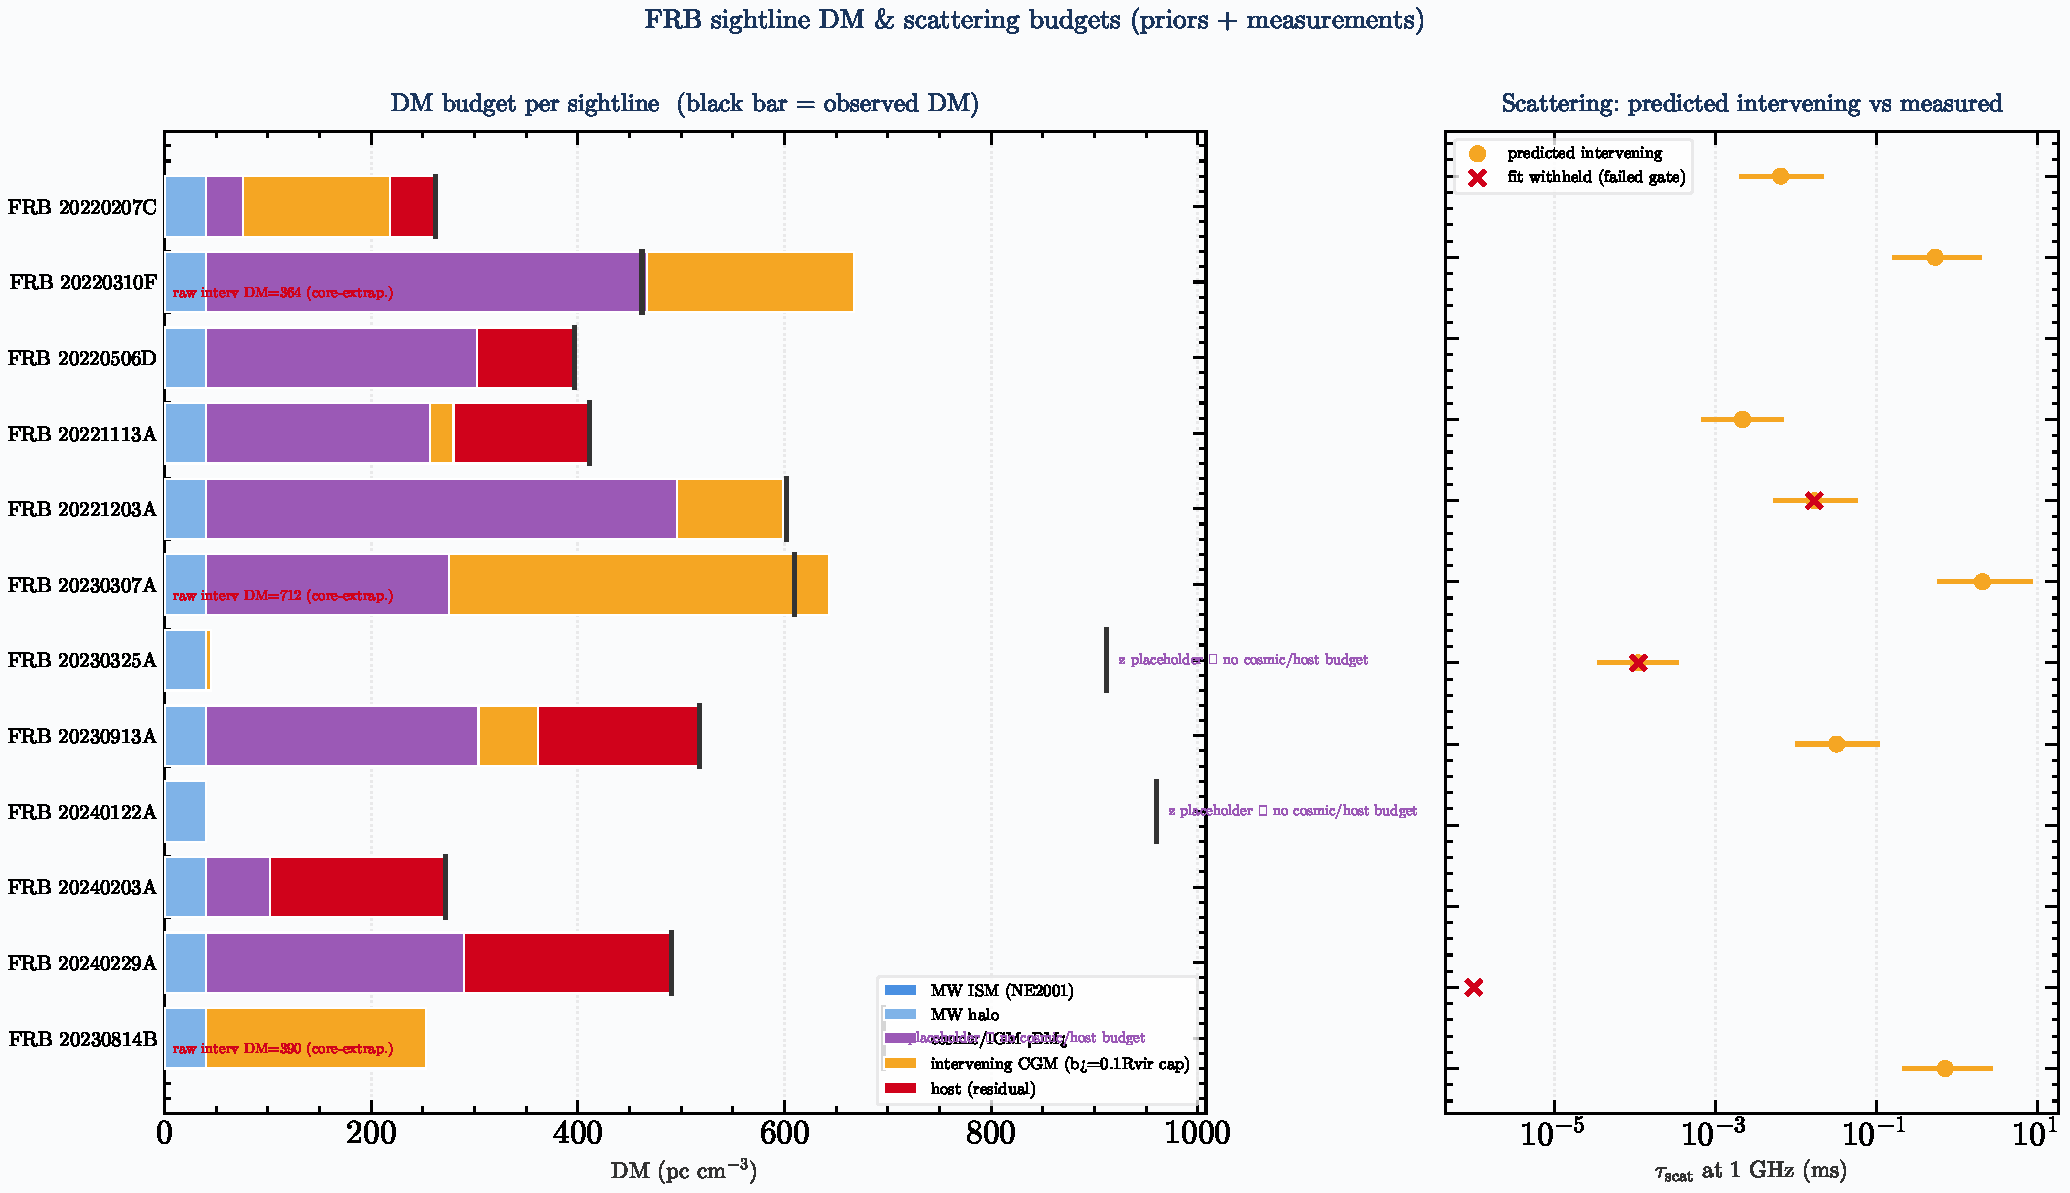
\includegraphics[width=0.95\textwidth]{sightline_dm_scattering_budget}
  \caption{Per-sightline dispersion and scattering budget for the twelve
  co-detections. \emph{Left:} the observed dispersion measure (black bar) of each
  burst decomposed into the Milky-Way ISM (NE2001) and halo, the cosmological mean
  (Macquart relation), the capped intervening circumgalactic column
  ($b<0.1\,R_{\mathrm{vir}}$), and the host residual; the placeholder-redshift
  sightlines (FRB 20230325A, FRB 20240122A, FRB 20230814B) show only the redshift-independent Galactic
  term. \emph{Right:} the predicted intervening pulse-broadening at $1\,\mathrm{GHz}$
  per sightline; the per-sightline measured $\tau$ from the uniform re-fit
  (Table~\ref{tab:beta}, Section~\ref{sec:results-alpha}) are not yet overlaid on
  this figure, so only the predicted contribution is shown here.
  Generated by the \texttt{dsa110-FLITS} pipeline
  (\texttt{galaxies/foreground/sightline\_budget.py}).}
  \label{fig:budget}
\end{figure*}

\FloatBarrier
\subsection{Turbulence spectrum and burst multiplicity}
\label{sec:results-alpha}

Across the twelve co-detected sightlines, the joint $\beta$-based fit
(Section~\ref{sec:jointfit}) constrains the turbulence spectral index for the
sightlines listed in Table~\ref{tab:beta}. For the well-constrained sightlines,
the recovered $\beta$---and the derived PBF shape and frequency-scaling index
$\alpha=2\beta/(\beta-2)$ that follow from it---are internally consistent by
construction. The Kolmogorov value $\beta=11/3$ ($\alpha\approx4.4$) and the
square-law limit $\beta=4$ ($\alpha=4$, exponential PBF) are specific points in
the continuous $\beta$ parameter space. Three sightlines are withheld from the
index sample: FRB~20221113A and FRB~20240122A return DSA-110 non-detections of
scattering, so $\beta$ rails to a prior bound and is unconstrained; and
FRB~20230913A is non-identifiable, because its single DSA-110 component cannot
be uniquely associated with one of the multiple CHIME sub-pulses---its DSA-110
arrival-time uncertainty ($\pm2.4\,\mathrm{ms}$) exceeds the CHIME sub-pulse
span ($1.0\,\mathrm{ms}$)---which leaves $\beta$ bimodal between the shallow and
steep prior rails. Population-level counts and median $\beta$ remain qualitative
pending FINAL figure regeneration; fixed-s² grids now adjudicate component
counts for FRB~20220506D (C2D1 favored), FRB~20221113A (C2D1 favored),
FRB~20240122A (weak C2D1 preference), and FRB~20230307A (C3D3 not robust over
C3D2).

% Rows generated by pipeline/analysis/beta_campaign/export_beta_table.py from
% beta_campaign_verdicts.json (beta-coherent thin-screen campaign, pass 1;
% pinned pipeline commit). Do not hand-edit values; notemarks a-d are
% annotation only.
\begin{deluxetable*}{lccccc}
\tablecaption{Turbulence spectral index $\beta$ from the uniform $\beta$-based
joint re-fit (Section~\ref{sec:jointfit}) of the co-detected sample. Eleven of
the twelve sightlines are listed; FRB~20240203A is excluded by the joint-fit
quality gate (catastrophic per-band misfit, $\chi^2_\nu=11.6/9.3$). The PBF
shape and the frequency-scaling index $\alpha=2\beta/(\beta-2)$ are both
derived from $\beta$ at each likelihood evaluation (thin-screen co-model).
$\tau_{1\,\mathrm{GHz}}$ is the shared pulse-broadening time referred to
$1\,\mathrm{GHz}$; $C\times D$ is the number of temporal components modeled in
the CHIME and DSA-110 bands. The Kolmogorov value is $\beta=11/3$
($\alpha\approx4.4$); the square-law limit is $\beta=4$ ($\alpha=4$,
exponential PBF). Two sightlines return interior posteriors (a measured
$\beta$ with 16th/84th-percentile uncertainties); the remaining nine rail at
the $\beta=4$ bound\tablenotemark{d}. All fits are verified against their
posterior-predictive checks; rows with an elevated single-band $\chi^2_\nu$
(FRB~20221203A, FRB~20230913A, FRB~20220207C) are provisional pending a
per-band systematics pass.
\label{tab:beta}}
\tablehead{\colhead{Burst} & \colhead{$C\times D$} & \colhead{$\beta$} &
  \colhead{$\alpha$ (derived)} & \colhead{$\tau_{1\,\mathrm{GHz}}$ [ms]} &
  \colhead{$\chi^2_\nu$ (C/D)}}
\startdata
FRB 20230325A\tablenotemark{a} & $1\times1$ & $3.722^{+0.014}_{-0.015}$ & $4.32^{+0.02}_{-0.02}$ & $0.119$ & 1.29/1.03 \\
FRB 20240229A & $1\times1$ & $\to 4$\tablenotemark{d} & $4$ (limit) & $0.0186$ & 1.57/1.02 \\
FRB 20221203A\tablenotemark{b} & $1\times1$ & $\to 4$\tablenotemark{d} & $4$ (limit) & $0.269$ & 1.57/6.73 \\
FRB 20230913A & $1\times1$ & $\to 4$\tablenotemark{d} & $4$ (limit) & $0.0245$ & 3.96/1.00 \\
FRB 20240122A & $1\times1$ & $\to 4$\tablenotemark{d} & $4$ (limit) & $0.219$ & 1.04/0.90 \\
FRB 20220207C & $1\times1$ & $\to 4$\tablenotemark{d} & $4$ (limit) & $0.294$ & 2.51/1.31 \\
FRB 20220506D & $2\times1$ & $\to 4$\tablenotemark{d} & $4$ (limit) & $0.843$ & 1.02/1.22 \\
FRB 20221113A & $2\times1$ & $\to 4$\tablenotemark{d} & $4$ (limit) & $0.314$ & 1.05/0.91 \\
FRB 20230814B & $2\times1$ & $\to 4$\tablenotemark{d} & $4$ (limit) & $2.19$ & 1.09/1.27 \\
FRB 20220310F\tablenotemark{c} & $2\times2$ & $\to 4$\tablenotemark{d} & $4$ (limit) & $1.18$ & 1.09/1.42 \\
FRB 20230307A & $3\times3$ & $3.228^{+0.020}_{-0.018}$ & $5.26^{+0.05}_{-0.05}$ & $0.469$ & 1.06/1.24 \\
% excluded (not citable): FRB 20240203A (gate FAIL: L2 catastrophic chi2_C=11.59 chi2_D=9.25)
\enddata
\tablenotetext{a}{Interior posterior near the Kolmogorov point; well fit in
both bands, so the measurement is a constraint rather than a prior-rail
artifact.}
\tablenotetext{b}{The elevated DSA-110 $\chi^2_\nu$ is a coherent shape misfit
localized at the bright pulse peak---off-peak residuals are white (RMS $\approx1$)
while the on-peak frequency-summed whitened residual reaches $\pm15\sigma$---where
a single scattered component does not fully reproduce the DSA-110 pulse shape.
The rail classification is nonetheless robust to the intrinsic-width
parametrization.}
\tablenotetext{c}{Multiplicity exemplar: C2D2 fit after local re-prep
(Section~\ref{sec:results-alpha}, Figure~\ref{fig:whitney_mult}). Fixed-s²
evidence confirms the second DSA-110 component.}
\tablenotetext{d}{Posterior railed at the $\beta=4$ prior bound (by the
$3\sigma$-proximity or $\ge30\%$ edge-mass criterion): the sightline is
consistent with square-law statistics and an exponential PBF, and $\alpha=4$
is quotable only as a geometry-conditioned limit under the thin-screen
closure, not as a measurement. An extended-medium PBF family may fit these
sightlines without railing; that re-analysis is deferred.}
\end{deluxetable*}


A subset of our co-detected bursts resolves into more than one temporal
component \citep{Pleunis2021}, and in these cases the inferred turbulence
spectrum depends on whether that multiplicity is modeled. The clearest case is
FRB~20220310F, whose DSA-110 profile resolves into two narrow sub-pulses
$0.34$\,ms apart while its CHIME/FRB profile is a broad, multi-peaked burst
that fails the residual-whiteness gate. A fit that models only one DSA-110
component cannot place a single scattered pulse under both sub-pulses and the
broad CHIME burst at once, and the shared $\beta$ rails against a prior
bound, leaving strong correlated residuals at both sub-pulse times
(Figure~\ref{fig:whitney_mult}, top; DSA whitened $\chi^2_\nu=16.1$). Adding
the second DSA-110 component is favored decisively and, critically,
\emph{stably}: on the matched-normalization grid the evidence gain is
$\Delta\ln Z\approx+2.7\times10^{3}$ and flat across the gain-prior variance
($+2706/+2683/+2671$ at $s^2=1/10/100$), so the component is real rather than
an artifact of the prior. With the second component in place, the fit unrails
to a well-constrained $\beta$ with white residuals in both bands
(Figure~\ref{fig:whitney_mult}, bottom; $\chi^2_\nu=1.1$ and $1.5$). The
inferred turbulence spectrum for this burst depends strongly on the
multiplicity: a missing sub-component drives $\beta$ to a prior rail,
distorting both the fitted PBF shape and $\alpha$ simultaneously. This
sensitivity does not afflict the well-constrained single-screen sightlines,
whose $\beta$ shift by $\le0.1$ in derived $\alpha$ under the same choices,
but it makes plain that multiplicity must be fixed before a marginal burst's
turbulence spectrum is quoted.

\begin{figure*}[!t]
  \centering
  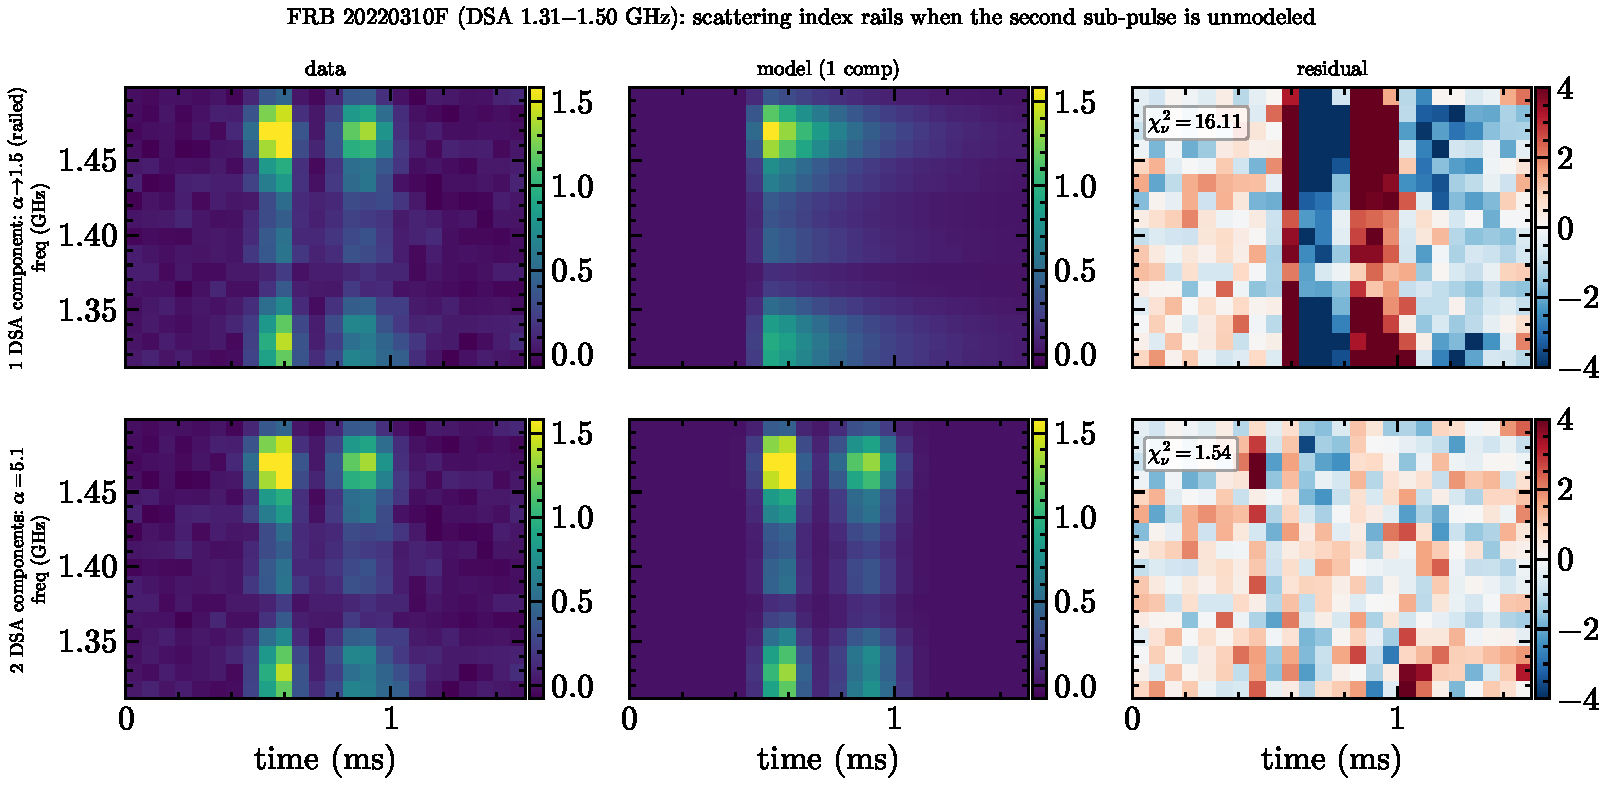
\includegraphics[width=0.92\textwidth]{whitney_multiplicity}
  \caption{Burst multiplicity drives the recovered turbulence spectrum for
  FRB~20220310F, shown in the DSA-110 band ($1.31$--$1.50\,\mathrm{GHz}$, where
  the two sub-pulses are resolved). \emph{Top:} a single DSA-110 component
  forces one heavily scattered pulse to span both $0.34$\,ms sub-pulses, railing
  the shared $\beta$ to a prior bound and leaving strong correlated residuals at
  both sub-pulse times (whitened $\chi^2_\nu=16.1$). \emph{Bottom:} adding the
  second component reproduces both sub-pulses, whitens the residual
  ($\chi^2_\nu=1.5$), and unrails $\beta$ to a well-constrained value. Both
  rows use the $\beta$-derived PBF of Section~\ref{sec:jointfit}; columns are
  the data, the gain-marginal model reconstruction, and the whitened residual on
  a common scale. Rendered from the provisional-citable joint fits and
  regenerated in FINAL form by the \texttt{dsa110-FLITS} joint-fit pipeline.}
  \label{fig:whitney_mult}
\end{figure*}

\FloatBarrier
\subsection{Isotropic-equivalent energies}
\label{sec:burst-energies}

For each sightline with a spectroscopic host redshift and a quality-passing joint
fit we estimate the isotropic-equivalent burst energy directly from the joint
CHIME--DSA fit,
without extrapolating either band's spectrum beyond where it is constrained.
The joint fit returns a per-band spectral amplitude and index,
$F_X(\nu) = c_{0,X}\,(\nu/\nu_{\mathrm{ref},X})^{\gamma_X}$, which we place on an
absolute scale with each telescope's per-channel radiometer conversion
$\sigma_{S,X}(\nu) = \mathrm{SEFD}_X(\nu)\,/\,[\sqrt{n_{\mathrm{pol}}\,\Delta\nu\,\Delta t}\,G_X(\nu)]$,
taking the system-equivalent flux density and primary-beam gain $G_X$ from the
DSA-110 \citep{Law2024} and CHIME/FRB \citep{CHIMEFRB2018,Michilli2021} flux
scales, and integrate over each instrument's observing band---CHIME over
$0.400$--$0.800\,\mathrm{GHz}$ and DSA over $1.311$--$1.499\,\mathrm{GHz}$,
%
\begin{equation}
E_{\mathrm{iso}} = \frac{4\pi D_L^2(z)}{1+z}\left[
  \int_{\nu_1^{C}}^{\nu_2^{C}} s_C\,F_{\mathrm{CHIME}}(\nu)\,d\nu
  + \int_{\nu_1^{D}}^{\nu_2^{D}} s_D\,F_{\mathrm{DSA}}(\nu)\,d\nu
\right],
\label{eq:eiso}
\end{equation}
%
with $D_L(z)$ from the fiducial \textit{Planck}\,2018 cosmology
\citep{Planck2018}, the $(1+z)$ bandwidth k-correction applied, and
$1\,\mathrm{Jy\,ms\,Hz} = 10^{-29}\,\mathrm{J\,m^{-2}}$. Bursts whose hosts lack
a spectroscopic redshift or for which no joint $c_0,\gamma$ fit exists are omitted
(Table~\ref{tab:burst-energies} caption). This band-restricted integral constrains
the energy released \emph{within the observed spectral envelope}: it avoids the
large, model-dependent extrapolation that a single power-law fit across the full
$0.4$--$1.5\,\mathrm{GHz}$ span would require, at the cost of not counting flux in
the unobserved $0.8$--$1.3\,\mathrm{GHz}$ gap, so the tabulated values are lower
limits on the total $0.4$--$1.5\,\mathrm{GHz}$ energy
(Table~\ref{tab:burst-energies}). The most distant sightline, FRB 20221203A
($z=0.51$), reaches $E_{\mathrm{iso}}\simeq1.1\times10^{41}\,\mathrm{erg}$, at the
luminous end of the co-detected sample. The absolute flux scale is anchored to the DSA-110 catalog \citep{Law2024} for
FRB~20220207C, which reproduces the catalog value to within a factor of two; the
remaining bands rely on the radiometer model without an independent catalog
cross-check, so their energies carry the additional, unquantified systematic of
the absolute scale.

\begin{deluxetable*}{lccccc}
\tablecaption{Isotropic-equivalent energies of the co-detected FRBs, integrated
over the CHIME ($0.4$--$0.8\,\mathrm{GHz}$) and DSA ($1.31$--$1.50\,\mathrm{GHz}$)
bands from the joint scattering fit and placed on an absolute scale with each
band's radiometer flux calibration. $\gamma_C,\gamma_D$ are the per-band spectral
indices; $E_{\mathrm{iso}}$ includes the $(1+z)$ k-correction. The quoted
$1\sigma$ uncertainty combines the per-band $c_0$ posterior width with the
absolute-scale systematic (SEFD and primary beam, ${\sim}0.25$ dex for CHIME and
${\sim}0.20$ dex for DSA), added in quadrature across the two bands. Eight of twelve
co-detections are tabulated. Excluded: FRB~20240229A (no joint $c_0,\gamma$ fit);
FRB~20230325A, FRB~20240122A, FRB~20230814B (no spectroscopic host redshift).
Per-band $c_0,\gamma$ amplitudes use the mixed-legacy joint-fit export (Pass 2
N=8 roster); all-exp scattering-only HPCC fits do not yet supply $c_0,\gamma$.
\label{tab:burst-energies}}
\tablehead{\colhead{Burst} & \colhead{$z$} & \colhead{$D_L$ [Mpc]} &
  \colhead{$\gamma_C$} & \colhead{$\gamma_D$} & \colhead{$E_{\mathrm{iso}}$ [erg]}}
\startdata
FRB 20240203A\tablenotemark{a} & $0.0740$ & $346$  & $-3.74$ & $-4.98$ & $(1.73 \pm 0.62)\times10^{39}$ \\
FRB 20230913A\tablenotemark{a} & $0.3024$ & $1617$ & $-1.81$ & $-4.91$ & $(6.71 \pm 2.68)\times10^{39}$ \\
FRB 20221113A & $0.2505$ & $1304$ & $-4.82$ & $+0.95$ & $(4.20 \pm 2.51)\times10^{40}$ \\
FRB 20220506D & $0.3005$ & $1606$ & $-4.48$ & $-4.85$ & $(4.30 \pm 2.29)\times10^{40}$ \\
FRB 20230307A & $0.2710$ & $1426$ & $-2.45$ & $-5.00$ & $(1.85 \pm 0.68)\times10^{40}$ \\
FRB 20220310F & $0.4790$ & $2774$ & $-1.00$ & $+2.91$ & $(7.24 \pm 3.06)\times10^{40}$ \\
FRB 20221203A & $0.5100$ & $2990$ & $+0.95$ & $-1.99$ & $(1.11 \pm 0.47)\times10^{41}$ \\
FRB 20220207C & $0.0430$ & $197$  & $-3.38$ & $-4.95$ & $(4.60 \pm 1.84)\times10^{38}$ \\
\enddata
\tablenotetext{a}{Host redshift not yet published; value provisional (no host-galaxy
  spectroscopic redshift in the literature as of this writing).}
\end{deluxetable*}

\section{Discussion}
\label{sec:discussion}

This section interprets the scattering, scintillation, turbulence, and
energetics results sightline by sightline before returning to the
population-level claims; it is developed alongside those results.

\subsection{Physical interpretation}
\label{sec:disc-interpretation}

% TODO(disc-interpretation): Open with the small set of result statements that
% survive re-validation. State what each result means physically before making
% any sample-level claim. This paragraph should depend on, in order:
% 1. Section~\ref{sec:results-budget}: revalidated DM and scattering budgets.
% 2. Section~\ref{sec:dominant-systems}: trusted dominant foreground systems.
% 3. Section~\ref{sec:results-scintillation}: trusted scintillation constraints.
% 4. Section~\ref{sec:results-alpha}: trusted turbulence or morphology results.
% 5. Section~\ref{sec:burst-energies}: trusted energy measurements.
%
% Avoid restating the old revoked campaign results here. In particular, do not
% quote the retired host-dominated 10/11 comparison, the FRB 20230913A
% intervening attribution, scintillation-excess factors, rail-class tallies,
% alpha=4 limits, beta values, burst energies, or DM-budget residuals until the
% producing analysis has passed its trust-restoration gate.

\subsection{Screen attribution from the budget and scintillation constraints}
\label{sec:disc-screen-attribution}

% TODO(disc-screen-attribution): Explain how a screen attribution is made after
% the relevant Results entries exist. The logic should be:
% - first ask whether the Galactic contribution can explain the scattering;
% - then ask whether a validated foreground system can explain the scattering;
% - then use revalidated scintillation products to decide whether a one-screen
%   or two-screen interpretation is favored;
% - only then assign the remaining contribution to the host or to an unknown
%   intervening system.
%
% This subsection should turn the budget and scintillation products into a
% physical statement, not introduce new numbers. It should also name any
% sightline whose attribution remains coverage-limited or model-limited.
%
% The formal machinery for the one- vs two-screen decision is in
% Appendix~\ref{app:twoscreen}: the two-screen ACF product term and the
% m_tot -> sqrt(3) unresolved-regime signature (Eq. eq:sqrt3), the resolution
% power RP (Eq. eq:rp), and the screen-distance upper limit (Eq. eq:distance).
% When writing this subsection, cite Appendix~\ref{app:twoscreen} for the
% derivation. Reduced but detected MW modulation is evidence for partial
% resolution, not permission to saturate the inequality or quote a point
% distance. Any later distance posterior requires a calibrated RP likelihood
% with realization scatter and the MW-screen-distance uncertainty propagated.

One boundary condition for this attribution is now fixed by the CHIME-band
scintillation campaign (Section~\ref{sec:results-scintillation}). The
high-resolution FRB~20240203A product yields four qualified CHIME-band
decorrelation bandwidths, while one DSA-band point passes the full
qualification, $\gamma=0.446^{+0.239}_{-0.250}\,$MHz at $1328.24\,$MHz for
FRB~20220506D. Because those certified measurements belong to different
bursts, they do not supply a two-band frequency-scaling index or a common
$600\,$MHz $\Delta\nu_d$ anchor for any single sightline. The other 23 CHIME
products and the other DSA panels remain fit diagnostics rather than certified
bandwidth measurements.

The two-screen consistency test is not yet evaluable
(Table~\ref{tab:twoscreen-provisional}). The $\tau\,\Delta\nu_d$ product must
pair each DSA-band decorrelation bandwidth with a scattering time refit under
the same fixed convention---a single-exponential pulse-broadening function
with $\alpha$ fixed to 4---rather than with the free-$\alpha$ joint-fit
values, which serve the morphology audit and would mix two different $\tau$
definitions in one product. Those fixed-index refits do not yet exist. We
therefore report the seven otherwise eligible sightlines as pending rather
than compute screen products from an inconsistent $\tau$ track. Once the
refits exist, the calculation will evaluate $\tau(\nu)\,\Delta\nu_d$
separately at every clean narrow DSA component frequency, without imposing a
bandwidth power law, and compare it with the conservative common-screen
interval $0.1$--$2$. The largely uncalibrated DSA widths and the unavailable
full posterior covariance remain additional prerequisites. No two-screen,
screen-distance, or Galactic/host attribution is made from the current
products.

% Generated by scripts/build_provisional_propagation_tables.py; do not hand-edit.
\begin{deluxetable*}{lccccl}
\tablecaption{Provisional component-level screen-consistency products.\label{tab:twoscreen-provisional}}
\tablehead{\colhead{FRB} & \colhead{$N$} & \colhead{Median $\tau\Delta\nu_d$} & \colhead{Range} & \colhead{min$(P-\sigma_P)$} & \colhead{Inference}}
\startdata
20220310F & 1 & 3e+02 & 3e+02--3e+02 & 2.4e+02 & two-screen favored \\ 
20220506D & 4 & 4.2 & 1.5--26 & 0.45 & indeterminate \\ 
20221113A & 1 & 9.5 & 9.5--9.5 & 3.4 & two-screen favored \\ 
20230307A & 3 & 1.1e+02 & 36--2.5e+02 & 17 & two-screen favored \\ 
20230325A & 1 & 3.8e+02 & 3.8e+02--3.8e+02 & 2.4e+02 & two-screen favored \\ 
20230814B & 3 & 42 & 14--7.2e+02 & 9.8 & two-screen favored \\ 
20240122A & 3 & 99 & 46--4.7e+02 & 6.5 & two-screen favored \\ 
\enddata
\tablecomments{All values are best-so-far and provisional unless explicitly certified.}
\end{deluxetable*}


We next cross-match the provisional fitted-scattering values against the
validated foreground census of Section~\ref{sec:obs-fg}
(Table~\ref{tab:foreground-propagation-provisional}). This comparison does not
support a sample-wide association test: only seven propagation fits are
accepted, only two of the four sightlines with budget-eligible foreground
systems have accepted fits, and most foreground-negative sightlines lie outside
the deep-imaging footprints. Those zeros are censored rather than clean
foreground-free controls.

FRB~20230307A offers the strongest case for a partial foreground
contribution. Its sightline lies within the deep-imaging footprints and
intersects the confirmed cluster J115120.4+714435 at $b/R_{500}=0.83$ along
with three budget-eligible galaxy halos. The fiducial foreground model
predicts $\tau_{\rm int}=0.015$ ms, approximately 22\% of the provisional
$\tau_{1\,\mathrm{GHz}}=0.0676$ ms: the identified structures could supply
part of the observed broadening, but not all of it under the current model.
If a future two-screen result computed under the fixed-index convention
supports multiple propagation layers, this foreground complex would be a
candidate scattering screen; the present data neither assign a scintillation
screen to it nor determine a screen distance.

The confirmed halo approximately 101 kpc from the FRB~20220310F sightline
intersects it geometrically, but its fiducial scattering contribution is only
about 0.5\% of the provisional fitted value, disfavoring a dominant causal
role.
Conversely, FRBs~20221113A and 20230325A have close projected but inconclusive
candidates at 16 and 60 kpc, respectively; redshift validation is required
before either can enter the foreground budget. FRBs~20240229A and 20240203A
contain confirmed foreground halos but lack accepted propagation fits. For
FRB~20240229A the fiducial foreground prediction exceeds the retained
morphology-only fit value by a factor of about 11, which is a fit--budget tension
to resolve rather than evidence for causation.

\input{foreground_propagation_provisional_table}

\subsection{Event-by-event interpretation ledger}
\label{sec:disc-sightline-ledger}

Each co-detection should receive a short interpretation only after its relevant
budget, foreground, scintillation, fit, and energy entries have been restored.

% TODO(disc-zach / FRB 20220207C): Interpret after revalidation. Check whether
% the restored budget gives a foreground, host, Galactic, or unresolved
% attribution; state any coverage or fit-quality caveat.

% TODO(disc-whitney / FRB 20220310F): Interpret after revalidation. This slot
% should connect the multi-component modeling decision to any budget, screen, or
% energy statement that survives the new analysis.

% TODO(disc-oran / FRB 20220506D): Interpret after revalidation. Make the survey
% coverage status explicit before saying whether the lack of a foreground term
% is informative.

% TODO(disc-isha / FRB 20221113A): Interpret after revalidation. Separate the
% foreground-census meaning from any scattering-fit or energy result.

% TODO(disc-wilhelm / FRB 20221203A): Interpret after revalidation. Do not reuse
% the old scintillation or negative-residual language unless both strands are
% re-established.

% TODO(disc-phineas / FRB 20230307A): Interpret after revalidation. If the
% restored analysis finds multiple foreground systems or a cluster contribution,
% explain which ingredient dominates and which is secondary.

% TODO(disc-freya / FRB 20230325A): Interpret after revalidation. Keep any
% redshift-placeholder limitation explicit before using this event in
% distance-dependent statements.

% TODO(disc-johndoeii / FRB 20230814B): Interpret after revalidation. The
% legacy galaxy-interior classification did NOT survive the V4 census (no
% registered candidates; DM_int=0, note u — see FLITS PR #183); host z is the
% provisional internal 0.5535 (Verdi et al. in prep.), and the source is a
% repeater (earlier DSA-only detection, data unsaved);
% interpret from association, DM, and coverage information alone.

% TODO(disc-hamilton / FRB 20230913A): Interpret after revalidation. Treat the
% intervening-screen claim as open until the foreground, budget, scattering, and
% scintillation strands all independently pass trust restoration.

% TODO(disc-mahi / FRB 20240122A): Interpret after revalidation. State the
% coverage limitation before using any zero-foreground or host statement.

% TODO(disc-chromatica / FRB 20240203A): Interpret after revalidation. If a
% quality gate still fails, explain what can be said from association, DM, and
% foreground information alone.

% TODO(disc-casey / FRB 20240229A): Interpret after revalidation. State whether
% this sightline is used as a clean comparison case, a budget constraint, or an
% energy-only point.

\subsection{Burst morphology as a systematic on the turbulence spectrum}
\label{sec:disc-alpha}

% TODO(disc-alpha): Rebuild this subsection only after Section~\ref{sec:results-alpha}
% contains trusted fit results. The interpretation should distinguish:
% - what is learned about burst morphology;
% - what is learned about the scattering geometry;
% - what is learned about the turbulence spectrum;
% - which claims are method diagnostics rather than sky measurements.
%
% Do not quote old beta values, alpha limits, rail classes, class fractions, or
% the retired multiplicity-bias demonstration as results. If a revalidated
% multi-component case remains, explain why the extra component changes the
% physical interpretation rather than merely improving the fit statistic.

\subsection{Energy interpretation}
\label{sec:disc-energies}

% Scoped 2026-07-15 (V3 session; validation-v3-energetics-2026-07-15.md).
% Structure below is settled; sentences marked [FILL] take numbers from the
% regenerated (data-driven) burst_energies.json after owner V3 clearance.
% Do not quote legacy c0/gamma-derived energies or any per-band spectral
% index from the revoked fits anywhere in this subsection.

% Draft lead-in — uncomment with the five scoped paragraphs after V3 clears.
%The band-restricted energies of Section~\ref{sec:burst-energies} are
%deliberately conservative objects: each is the energy radiated within the
%two observed spectral windows, computed from the calibrated channel data with
%no spectral model, no extrapolation across the unobserved
%$0.8$--$1.3\,$GHz gap, and no fitted parameter inherited from the scattering
%analysis. Their limitations separate cleanly into five categories that we
%keep distinct.
%
% (1) Calibration. The absolute scale is catalog-anchored for three
% sightlines (~2x confidence) and radiometer-model-trusted for the rest;
% the 0.20-0.25 dex systematics dominate every row's error budget. No
% ranking of two rows closer than ~a factor of 2 is meaningful.
%
% (2) Spectral shape. In-band indices are unconstrained by design (narrow
% fractional bands; the DSA-band steepness the fits kept railing on is a
% model-family statement, not a measurement — cite the descriptive finding
% only if/when the C1 campaign re-establishes it). The two-band partition
% E_C vs E_D is the one shape-like quantity we CAN discuss: [FILL] state
% the observed E_C/E_D range; interpret order-unity scatter as evidence of
% per-burst spectral-envelope diversity across the octave gap, while noting
% that scintillation modulation and beam-model error enter that ratio and
% cannot be separated from intrinsic narrowbandedness until the two-band
% scintillation campaign concludes (Section~\ref{sec:disc-screen-attribution}).
%
% (3) Host redshift. Two provisional-z rows (FRBs 20230913A, 20240203A):
% any population-facing sentence must survive their removal; check and say
% so explicitly ([FILL] after table lands).
%
% (4) Selection. Co-detection requires threshold crossings at BOTH 600 MHz
% and 1.4 GHz: the sample is biased toward bursts that are simultaneously
% bright across the octave, i.e. against strongly banded events. The energy
% rows are therefore not a fair draw from either instrument's fluence
% function, and no luminosity-function normalization should be attempted
% from them. What CAN be said: [FILL] the span of ~3 decades in E_iso within
% a co-detected sample shows the joint-detection criterion still admits a
% wide intrinsic energy range, with the low end (~1e38-1e39 erg at
% z < 0.08 — zach, chromatica) illustrating that the local volume
% contributes the faint tail, consistent with the strong E-z selection
% correlation expected for flux-limited surveys. A qualitative comparison to
% the CHIME/FRB first-catalog energy distribution (Shin et al. 2023) is
% appropriate ONLY as an order-of-magnitude placement, with the band
% non-comparability caveat stated in the same sentence.
%
% (5) Forward link (lane E2 seed). Energies are the propagation-independent
% axis of the synthesis: fluence is conserved under scattering to first
% order, so E_iso vs (DM_host residual, tau, foreground class) scatter plots
% separate intrinsic brightness from path effects. With 8 rows this stays
% qualitative — frame as "no evident correlation" / "consistent with
% independence" unless something dramatic appears; a real statement needs
% the C1-re-fit tau values (gate: post-C, lane E2).

\subsection{Population limits and selection effects}
\label{sec:disc-population-limits}

% TODO(disc-population-limits): State which sample denominator applies to each
% claim. The twelve co-detections are the full association sample, but budget,
% foreground, scintillation, turbulence, and energy claims each have their own
% validated subset and exclusion reasons.
%
% Use this subsection to prevent over-reading the sample. Discuss redshift
% incompleteness, foreground-catalog coverage, fit-quality gates, and band
% selection effects only after the relevant Results text has named the affected
% sightlines.

\subsection{Implications for the next analysis pass}
\label{sec:disc-next-pass}

% TODO(disc-next-pass): Close the Discussion by naming the analysis that the
% revalidated results require next. Candidate topics include geometry selection,
% two-screen treatment, foreground-census sensitivity, burst-morphology
% modeling, or energy-selection rules. The closing paragraph should follow from
% the restored Results, not from the revoked campaign narrative.

\section{Conclusions}
\label{sec:conclusions}

% TODO: summary of the per-sightline attribution and what co-detection adds.


\appendix
\section{Per-burst association cards}
\label{app:assoc-cards}

Figures~\ref{fig:assoc_grid_a} and~\ref{fig:assoc_grid_b} reproduce the per-burst timing
residual, independent DM comparison (where available), and positional agreement
diagnostics summarized in Table~\ref{tab:toa}, arranged as six cards per page in a
two-column grid.

% Figure provenance lives in sections/association_cards.tex with the figure
% blocks, because that file owns the includegraphics calls and card roster.
% Per-burst association cards are intentionally not included in the manuscript
% until the association and DM-observation re-validation pass is complete.
%
% Removed figure candidates:
% - Artifacts: figures/association_cards/association_card_*.pdf
% - Generator: pipeline/crossmatching/plot_association_cards.py
% - Inputs:
%   pipeline/crossmatching/toa_crossmatch_results.json
%   pipeline/crossmatching/association_report.json
%   pipeline/crossmatching/chime_side_inputs.json
%   pipeline/crossmatching/notebook_reproduction_fixture.json
% - Regeneration command: from pipeline/, run
%   `python crossmatching/plot_association_cards.py`; the script writes
%   crossmatching/association_cards/*.pdf and copies the PDFs to
%   figures/association_cards/.
% - Reason withheld: these figures summarize association timing, independent
%   DM, and position diagnostics; those products are revoked until V6 restores
%   trust.


\FloatBarrier

% The exponential-PBF appendix is parked for this circulation draft because the
% manuscript is not yet ready to quote any alpha-limit result language.
% \section{An exponential pulse-broadening function implies $\alpha=4$}
\label{app:emg-alpha4}

Exponentially modified Gaussian (EMG) profiles---a Gaussian pulse of width
$\sigma$ convolved with the one-sided exponential
$p(t)=\tau^{-1}e^{-t/\tau}$ ($t\ge0$)---are the standard phenomenological
scattering model in the pulsar and FRB literature, and they are the kernel our
pipeline evaluates in its exponential limit,
\begin{equation}
\label{eq:emg}
I(t)\;\propto\;\frac{1}{2\tau}\,
\exp\!\left[\frac{\sigma^{2}}{2\tau^{2}}-\frac{t-t_{0}}{\tau}\right]
\operatorname{erfc}\!\left[\frac{1}{\sqrt{2}}
\left(\frac{\sigma}{\tau}-\frac{t-t_{0}}{\sigma}\right)\right].
\end{equation}
This appendix records why adopting an EMG kernel is not scaling-agnostic:
within thin-screen scattering the exponential pulse-broadening function (PBF)
is uniquely the $\beta=4$ member of the power-law family of
Section~\ref{sec:beta-scattering-methods}, and $\beta=4$ fixes $\alpha=4$.
Fixing $\alpha=4$ in an EMG fit is therefore a self-consistency requirement
rather than a modeling choice, and conversely an EMG fit with $\alpha$ free
combines incompatible turbulence assumptions.

\subsection{Uniqueness of the exponential limit}

For a thin screen with $P_n(q)\propto q^{-\beta}$, $2<\beta<4$, and a
negligible inner scale, the PBF is exponential at small delays and develops a
power-law tail at large delays \citep{Cordes2025}:
\begin{equation}
\label{eq:pbf-family}
p(s)\;\propto\;
\begin{cases}
e^{-s}, & s\le s_{c},\\[2pt]
e^{-s_{c}}\,(s/s_{c})^{-\beta/2}, & s>s_{c},
\end{cases}
\qquad
s_{c}=2\ln\!\frac{2}{4-\beta},
\end{equation}
with $s=t/\tau$. The fraction of the unit-normalized PBF carried by the tail
is
\begin{equation}
\label{eq:tailmass}
M(\beta)\;=\;
\int_{s_{c}}^{\infty} e^{-s_{c}}\!\left(\frac{s}{s_{c}}\right)^{-\beta/2} ds
\;=\;\frac{(4-\beta)^{2}\,s_{c}}{2\,(\beta-2)},
\end{equation}
which is strictly positive for every $2<\beta<4$ (e.g.\ $M(3)=\ln 2$) and
vanishes only in the limit $\beta\to4$, where $s_{c}\to\infty$ and the family
degenerates to the pure exponential. The tail is normalizable for $\beta>2$
while its mean delay converges only for $\beta>4$, so every $\beta<4$ member is
qualitatively heavier-tailed than the exponential rather than a small
perturbation of it. An exactly exponential PBF therefore corresponds to one and
only one point of the family: the square-law limit $\beta=4$.

\subsection{The scaling forced by $\beta=4$}

The same $\beta$ sets the frequency scaling. With the inertial-range phase
structure function $D_\phi(\rho)\propto\nu^{-2}\rho^{\beta-2}$
(Section~\ref{sec:beta-scattering-methods}), the diffractive scale defined by
$D_\phi(\rho_{\rm d})=1$ obeys $\rho_{\rm d}\propto\nu^{2/(\beta-2)}$, the
scattering angle scales as $\theta_{\rm d}\propto(k\rho_{\rm d})^{-1}\propto
\nu^{-\beta/(\beta-2)}$, and the geometric delay $\tau\propto\theta_{\rm d}^{2}$
gives
\begin{equation}
\label{eq:alpha-closure-appendix}
\tau\;\propto\;\nu^{-2\beta/(\beta-2)}
\quad\Longrightarrow\quad
\alpha(\beta)=\frac{2\beta}{\beta-2},
\qquad \alpha(4)=4 .
\end{equation}
An EMG kernel thus commits a fit to $\tau\propto\nu^{-4}$ by definition.

Three corollaries govern our fit design. First, the only fixed scattering index
consistent with an exponential kernel is $\alpha=4$; fixing the Kolmogorov
value $\alpha=22/5$ inside an EMG would be inconsistent, because $\beta=11/3$
implies the tailed PBF of Equation~\ref{eq:pbf-family}, not an exponential.
Second, an EMG fit with $\alpha$ free asserts $\beta=4$ through its shape while
asserting $\beta\neq4$ through its scaling; a shallow apparent index recovered
that way measures departure from the assumed scattering family---burst
morphology, an extended medium, or a finite inner scale
\citep{Bhat2004,Cordes2025}---rather than a turbulence spectral index. Third,
$\alpha=4$ is a two-sided \emph{floor} for the whole single-thin-screen family:
Equation~\ref{eq:alpha-closure-appendix} exceeds 4 for every $\beta<4$
($\alpha$ is monotonically decreasing in $\beta$), while for $\beta\ge4$ the
structure function saturates to the square-law form and pins
$\tau\propto\nu^{-4}$ regardless of $\beta$ \citep{Rickett1990}. An empirical
$\alpha<4$ is therefore unreachable within this family and must be read as a
violated assumption, never as a spectral index
(Section~\ref{sec:beta-scattering-methods}). This is
why our primary model samples $\beta$ directly and derives both the PBF shape
and $\alpha(\beta)$ from it (Section~\ref{sec:beta-scattering-methods}).

% The algebra in this appendix (closure values, limiting behavior, tail
% convergence conditions, and equivalences of the EMG forms) was verifiedf
% symbolically with WolframScript.


\bibliographystyle{aasjournal}
\bibliography{bib/refs}

\end{document}
